\documentclass[11pt,letterpaper]{article}

\newenvironment{proof}{\noindent{\bf Proof:}}{\qed\bigskip}

\newtheorem{theorem}{Theorem}
\newtheorem{corollary}{Corollary}
\newtheorem{lemma}{Lemma} 
\newtheorem{claim}{Claim}
\newtheorem{fact}{Fact}
\newtheorem{definition}{Definition}
\newtheorem{assumption}{Assumption}
\newtheorem{observation}{Observation}
\newtheorem{example}{Example}
\newcommand{\qed}{\rule{7pt}{7pt}}

\newcommand{\assignment}[5]{
\thispagestyle{plain} 
\newpage
\setcounter{page}{1}
\noindent
\begin{center}
\framebox{ \vbox{ \hbox to 6.28in
{\bf \textsf{ #1 \hfill #2 }}
\vspace{4mm}
\hbox to 6.28in
{\hspace{2.5in}\Large\mbox{\bf \textsf{Problem Set #3}}}
\vspace{4mm}
\hbox to 6.28in
{{\it Handed Out: #4 \hfill Due: #5}}
}}
\end{center}
}
%\assignment{CS224W: Social and Information Network Analysis}{Fall 2012}{$1$}{September $11^{th}$, $2012$}{September $20^{th}$, $2012$}

\newcommand{\normaldoc}[5]{
\thispagestyle{plain} 
\newpage
\setcounter{page}{1}
\noindent
\begin{center}
\framebox{ \vbox{ \hbox to 6.28in
{\bf \textsf{ #1 \hfill #2 }}
\vspace{4mm}
\hbox to 6.28in
{\hfill\Large\mbox{\bf \textsf{#3}}\hfill}
\vspace{4mm}
\hbox to 6.28in
{#4 \hfill {Completed Date:  \textit{#5} }}
}}
\end{center}
\markright{#4}
}

\newcommand{\project}[6]{
\thispagestyle{plain} 
\newpage
\setcounter{page}{1}
\noindent
\begin{center}
\framebox{ \vbox{ \hbox to 6.28in
{\bf \textsf{ #1 \hfill #2 }}
\vspace{4mm}
\hbox to 6.28in
{\hfill\Large\mbox{\bf \textsf{Project #3: #6}}\hfill}
\vspace{4mm}
\hbox to 6.28in
{#4 \hfill {\textit{#5} }}
}}
\end{center}
\markright{#4}
}

\newcommand{\solution}[5]{
\thispagestyle{plain} 
\newpage
\setcounter{page}{1}
\noindent
\begin{center}
\framebox{ \vbox{ \hbox to 6.28in
{\bf \textsf{ #1 \hfill #2 }}
\vspace{4mm}
\hbox to 6.28in
{\hspace{2.5in}\Large\mbox{\bf \textsf{Problem Set #3}}}
\vspace{4mm}
\hbox to 6.28in
{#4 \hfill {Completed Date: \textit{#5} }}
}}
\end{center}
\markright{#4}
}
%\solution{CS224W: Social and Information Network Analysis}{Fall 2012}{0}{Botao Hu (botaohu@stanford.edu)}{\today}

\newenvironment{algorithm}
{\begin{center}
\begin{tabular}{|l|}
\hline
\begin{minipage}{1in}
\begin{tabbing}
\quad\=\qquad\=\qquad\=\qquad\=\qquad\=\qquad\=\qquad\=\kill}
{\end{tabbing}
\end{minipage} \\
\hline
\end{tabular}
\end{center}}

\def\Comment#1{\textsf{\textsl{$\langle\!\langle$#1\/$\rangle\!\rangle$}}}


\usepackage{graphicx,amssymb,amsmath,enumerate}
\usepackage{courier}
\usepackage{color}
\usepackage{listings}
\usepackage{fancyvrb}
\usepackage{stmaryrd}

\definecolor{dkgreen}{rgb}{0,0.6,0}
\definecolor{gray}{rgb}{0.5,0.5,0.5}
\lstset{language=Python,
	frame=lines,
   basicstyle=\ttfamily\fontsize{8}{12}\selectfont,
   keywordstyle=\color{blue},
   commentstyle=\color{red},
   stringstyle=\color{dkgreen},
   numbers=left,
   numberstyle=\tiny\color{gray},
   stepnumber=1,
   numbersep=10pt,
   backgroundcolor=\color{white},
   tabsize=2,
   showspaces=false,
   showstringspaces=false,
   lineskip=-3.5pt }
\oddsidemargin 0in
\evensidemargin 0in
\textwidth 6.5in
\topmargin -0.5in
\textheight 9.0in

\begin{document}

\project{CS255: Introduction to Cryptography}{Winter 2013}{2}{Botao Hu (botaohu@stanford.edu), Borui Wang (borui@stanford.edu)}{\today}{SSL MiTM}

\pagestyle{myheadings}  % Leave this command alone

\section{Introduction}
We developed an SSL proxy that implements a man-in-the-middle (MiTM) attack on SSL. 
Our proxy is controlled an admin communication channel through a separate secure SSL connection. The client requires a password authentication to execute commands through the admin communication channel.

\begin{figure}[h!]
\centering
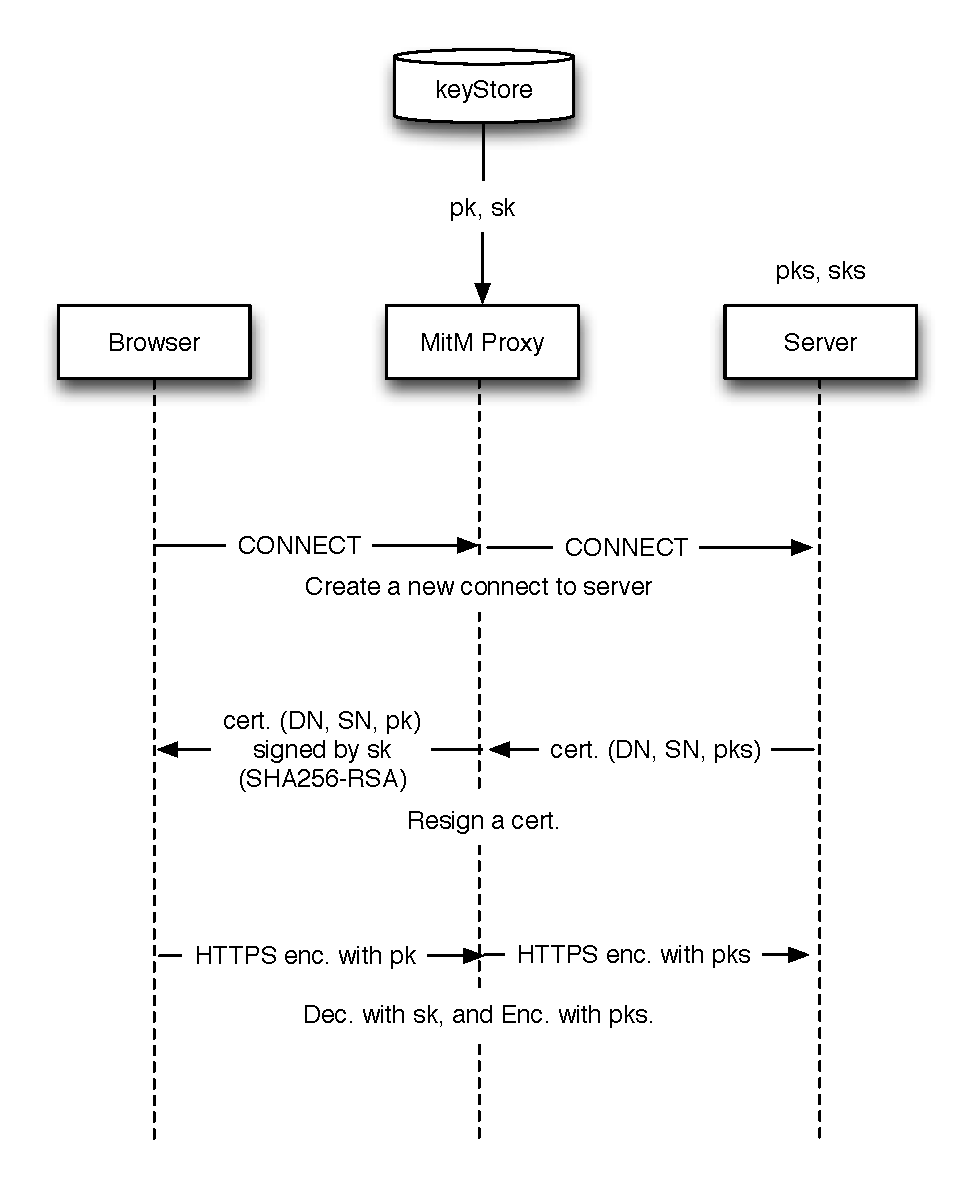
\includegraphics[width=0.7\textwidth]{proxy.eps}
\caption{Illustration of how MiTM proxy works}
\label{fig:diag}
\end{figure}


\section{Design}

\subsection{Key Generation}

First we generate a keyStore for the MITM's CA(issuer) information. We named our CA ``Very Secure Software'' with its location located at Cupertino, California, and we signed the private key using RSA algorithm. The keyStore is under the alias my key and it uses password  ``foobar'' for verification:

\begin{lstlisting} 
keytool -genkeypair -dname "CN=Very Secure Software, OU=Very Secure Software Group, 
    O=Very Secure Inc, L=Cupertino, S=California, C=US" -alias mykey -keypass <password> 
    -keystore ./keystore -storepass <storepassword> -validity 365 -keyalg RSA
\end{lstlisting}

\subsection{SSL MiTM}

To trick the browser into thinking that it receives a legit certificate from its intended remote server, we need to use the DN(such as the domain's common name, the organization name ,etc. ) and serial number of the original certificate from the remote site but changes its key into our public key, where the certificate is signed by our private key. 

In order to do so, whenever we receive a ssl CONNECT request, we send the same request to the remote server.  Once the server sends back its certificate to us, we look up and extract the DN and serial number of the certificate in the ssl session. Then we create a new certificate on the live that and make it appears to be issued to the same DN with the same serial number we get from the remote server. However, we add to the certificate the DN information of the issuer we created and its public key to make it appears to be issued by Very Secure Software. Then we sign the certificate using our private key with a deterministic algorithm (we use SHA256 with RSA) and send back our forged certificate to the browser. The browser will think that our certificate is from the remote site because it's DN matches the remote site's information and the verification on the certificate using the public key we provide is successful. 

The whole process is demostrated in the figure \ref{fig:diag}. 

\subsection{Admin Communication Channel \& Password Authentication} 
For the sever admin access, we generate a salted password hash using BCrypt and stored the value into pwdFile manually. 

The code adopting BCrypt library to generate a password hash and the salt is listed below. 
\begin{lstlisting}
  salt = BCrypt.gensalt();
  hash = BCrypt.hashpw(password, salt);
\end{lstlisting}

When the server starts, we read the hash and salt value from the pwdFile and later use it to verify if the provided admin password is correct by hashing the provided value with the salt and see if they equal to the hash value we have in pwdFile. 


\section{Steps to run}
\begin{enumerate}[(1)]
  \item Create a private key in a keystore by running 

\begin{lstlisting} 
keytool -genkeypair -dname "CN=Very Secure Software, OU=Very Secure Software Group, 
    O=Very Secure Inc, L=Cupertino, S=California, C=US" -alias mykey -keypass <password> 
    -keystore ./keystore -storepass <storepassword> -validity 365 -keyalg RSA
\end{lstlisting}

\item Run the SSL proxy server with the command 
\begin{lstlisting}
java -classpath ${CLASSPATH}:.:iaik_jce.jar mitm.MITMProxyServer 
    -keyStore keystore -keyStorePassword <storepassword> -pwdFile pwdFile -output
\end{lstlisting}

\item Send command to the admin server with the command 
\begin{lstlisting}
java -classpath ${CLASSPATH}:.:iaik_jce.jar mitm.MITMAdminClient -password <password> -cmd 
  <shutdown|stats>
\end{lstlisting}


\item Set the SSL proxy of your browser to localhost:8001.
\item Visit a https site with the browser.
\end{enumerate}


\section{Short Answers}

\begin{enumerate}[(1)]
\item Question: Suppose an attacker controls the network hardware and can intercept or redirect
messages. Show how such an attacker can control the admin server just as well as 
a legitimate admin client elsewhere on the network. Give a complete and specific description of the changes you would make to fix this vulnerability.

Answer:

An attacker can set a MiTM server between MiTMAdminServer and MiTMAdminCilent. 
If MiTMAdminCilent sends a request to MiTMAdminServer, the attacker will intercept this packet and obtain the user password, and then authenticate as admin client with his credentials, and then play as a MiTMAdminCilent to send to MiTMAdminServer the forged request with the correct password.

To fix it, we can adopt sig-based challenge response verfication, 
MiTMAdminServer will issue a challenge to the client, which they must then answer with a response that contained the signature of the message and the command signed by the cilent's secret signing key and then the server verifies their identity.
The MitM can not modify request packets as the client because he does not know the cilent's secret signing key.

\item Question: Suppose an attacker is trying to gain unauthorized access to your MITM server
by making its own queries to the admin interface. Consider the security of your
implementation against an attacker who (a) can read the admin server's password
file, but cannot write to it; (b) can read and/or write to the password file between
invocations of the admin server. 
For each threat model, either show that your implementation is secure, or give an attack. (N.B.: For full credit, your implementation should at least be secure under (a). 
What, if anything, would you need to change in order to make it secure under (b)? If your answer requires any additional cryptographic tools, you should fully specify them (including the names of any algorithms,
cryptosystems, and/or modes of operation that you would use.)

Answer: 

If an attacker can read the password hash file of the admin server, he know salt and hashed password, and so he can use dictionary attacks or bruteforce to get the password hash. But as long as we use a secure  and long password, the attack has to take a lot of time (say years) to recover the password.

If an attacker can write the password hash file of the admin server, he could simply replace the salt and hashed password with his own password hash and salt. Our implementation will be easily broken by this attack. To prevent this attack, we could sign the password file with a private key from the server that the attacker does not know. We could generate a new signing certificate by keytool. 

\item Question:
How would you change a web browser to make it less likely that an end user would be
fooled by a MITM attack like the one you have implemented? (This is an important
question to ask because when dealing with security, we never just build attacks: we
also need to think of ways to prevent them.)

Answer: 

A simple solution is to never accept certificate with an invalid certificate chains. 

For high security websites, we could adopt public key pinning technology in the browser to prevent MitM. This means that certificate chains for, say, \texttt{https://www.google.com}, must include a whitelisted public key. It's a fatal error otherwise. 


\end{enumerate}

\end{document}

